%HW10.tex
%
% Tenth Homework for Graduate Algebra
% Frank Sottile
%%%%%%%%%%%%%%%%%%%%%%%%%%%%%%%%%%%%%%%%%%%%%%%%%%%%%%%%%%%%%%%%%%%%%%%
\documentclass[12pt]{article}
\usepackage{multicol,amssymb,amsmath}
\usepackage{graphicx}
\usepackage{xcolor}
\headheight=8pt
%
\topmargin=-95pt
\textheight=744pt   \textwidth=575pt
\oddsidemargin=-60pt \evensidemargin=-60pt

\pagestyle{empty}

%%%%%%%%%%%%%%%%%%%%%%%%%%%%%%%%%%%%%%%%%%%%
\newcommand{\HH}{{\mathbb H}}
\newcommand{\FF}{{\mathbb F}}
\newcommand{\RR}{{\mathbb R}}
\newcommand{\CC}{{\mathbb C}}
\newcommand{\KK}{{\mathbb K}}
\newcommand{\NN}{{\mathbb N}}
\newcommand{\QQ}{{\mathbb Q}}
\newcommand{\TT}{{\mathbb T}}
\newcommand{\ZZ}{{\mathbb Z}}
\newcommand{\calA}{{\mathcal A}}
\newcommand{\calL}{{\mathcal L}}
\newcommand{\be}{{\bf e}}

\newcommand{\Hom}{\mbox{Hom}}
\newcommand{\End}{\mbox{End}}
\newcommand{\Mat}{\mbox{Mat}}
\newcommand{\rank}{\mbox{rank}}
\newcommand{\spec}{\mbox{spec}}
\newcommand{\cone}{\mbox{cone}}

\newcommand{\Square}{\raisebox{-2pt}{\includegraphics{figures/Square.eps}}}

\newcommand{\vect}[2]{(\begin{smallmatrix}#1\\#2\end{smallmatrix})}
\newcommand{\msp}{\hspace{8pt}}

\newcommand{\barsl}{\noindent\begin{minipage}[t]{575pt}
{\color{violet}\rule{575pt}{1.2pt}}\vspace{-5.7mm}\\
{\color{blue}\rule{575pt}{1.2pt}}\vspace{-5.7mm}\\
{\color{green}\rule{575pt}{1.2pt}}\vspace{-5.7mm}\\
{\color{yellow}\rule{575pt}{1.2pt}}\vspace{-5.7mm}\\
{\color{orange}\rule{575pt}{1.2pt}}\vspace{-5.7mm}\\
{\color{red}\rule{575pt}{1.2pt}}
\end{minipage}}


\def\demph#1{{\color{blue}{\sl #1}}}
\def\defcolor#1{{\color{blue}#1}}

\begin{document}
\LARGE 
\noindent
Algebra II\ \ Winter 2021 \hfill 23 March\makebox[40pt][l]{\ }\newline
Frank Sottile \hfill
\Large\sf
Tenth Homework\makebox[40pt][l]{\ }
\vspace{5pt}
\normalsize

\noindent
Write your answers neatly, in complete sentences, and prove all assertions.
Start each problem on a new page (this makes it easier in Gradescope).
Revise your work before handing it in, and submit a .pdf  created from a LaTeX source to Gradescope.
Correct and crisp proofs are greatly appreciated; oftentimes your work can be shortened and made clearer.

\noindent
{\color{red}Due Monday 29 March.}\vspace{1pt}

\barsl

\begin{enumerate}
%%%%%%%%%%%%%%%%%%%%%%%%%%%%%%%%%%%%%
%\setcounter{enumi}{52}

%\newpage
%%%%%%%%%%%%%%%%%%%%%%%%%%%%%%%%%%%%%%%%%%%%%%%%%%%%%%%%%%%%%%%%%%%%%%%%%%%%%%%%%
\item   Let $F/K$ be a field extension with intermediate fields $F_1,F_2$ that are finite extensions of $K$.
  \begin{enumerate}
  \item Write \defcolor{$F_1F_2$} for the subfield of $F$ generated by  $F_1$ and $F_2$.
    Prove that $[F_1F_2\colon K]\leq[F_1\colon K]\cdot[F_2\colon K]$
    
    (Hint: Let $\alpha_1,\dotsc\alpha_n$ be a basis for $F_1$ over $K$ and write $F_1=K(\alpha_1,\dotsc\alpha_n)$, and the same for $F_2$.)

  \item If the two indices $[F_1\colon K]$ and $[F_2\colon K]$  are relatively prime, show that we obtain an equality in part (a).

  \end{enumerate}
  \vspace{-2pt}
%%%%%%%%%%%%%%%%%%%%%%%%%%%%%%%%%%%%%%%%%%%%%%%%%%%%%%%%%%%%%%%%%%%%%%%%%%%%%%%%%


%\newpage
%%%%%%%%%%%%%%%%%%%%%%%%%%%%%%%%%%%%%%%%%%%%%%%%%%%%%%%%%%%%%%%%%%%%%%%%%%%%%%%%%
\item    Let $F/K$ be a field extension.
  If $u\in F$ is algebraic over $K$ of odd degree, then so is $u^2$, and $K(u)=K(u^2)$.
\vspace{-2pt}
%%%%%%%%%%%%%%%%%%%%%%%%%%%%%%%%%%%%%%%%%%%%%%%%%%%%%%%%%%%%%%%%%%%%%%%%%%%%%%%%%

%\newpage
%%%%%%%%%%%%%%%%%%%%%%%%%%%%%%%%%%%%%%%%%%%%%%%%%%%%%%%%%%%%%%%%%%%%%%%%%%%%%%%%%
\item   (a) Let $F:=\QQ(\sqrt{2},\sqrt{3})$.
  Determine $[F\colon\QQ]$ and give a basis of $F$ over $\QQ$.

  (b) Do the same for $F:=\QQ(\sqrt{-1},\sqrt{3},\omega)$, where $\omega\neq 1$ is a cube root of $1$.
\vspace{-2pt}
%%%%%%%%%%%%%%%%%%%%%%%%%%%%%%%%%%%%%%%%%%%%%%%%%%%%%%%%%%%%%%%%%%%%%%%%%%%%%%%%%

%\newpage
%%%%%%%%%%%%%%%%%%%%%%%%%%%%%%%%%%%%%%%%%%%%%%%%%%%%%%%%%%%%%%%%%%%%%%%%%%%%%%%%%
\item Let $K$ be a field and $x_1,\dotsc,x_n$ indeterminates.
  Let $u$ be an element of the function field $K(x_1,\dotsc,x_n)$.

  Show that either $u\in K$ or $u$ is transcendental over $K$.
\vspace{-2pt}
%%%%%%%%%%%%%%%%%%%%%%%%%%%%%%%%%%%%%%%%%%%%%%%%%%%%%%%%%%%%%%%%%%%%%%%%%%%%%%%%%

%\newpage
%%%%%%%%%%%%%%%%%%%%%%%%%%%%%%%%%%%%%%%%%%%%%%%%%%%%%%%%%%%%%%%%%%%%%%%%%%%%%%%%%
\item   Let $u=x^4/(x^2+1)$ be an element of the function field $\CC(x)$.
  Show that $\CC(x)$ is a simple algebraic extension of $\CC(u)$, and determine the degree of this extension.
\vspace{-2pt}
%%%%%%%%%%%%%%%%%%%%%%%%%%%%%%%%%%%%%%%%%%%%%%%%%%%%%%%%%%%%%%%%%%%%%%%%%%%%%%%%%

%\newpage
%%%%%%%%%%%%%%%%%%%%%%%%%%%%%%%%%%%%%%%%%%%%%%%%%%%%%%%%%%%%%%%%%%%%%%%%%%%%%%%%%
\item   Let $F/K$ be a field extension, with intermediate fields $F_1,F_2$ that are Galois extensions of $K$.
  \begin{enumerate}
  \item Show that $F_1\cap F_2$ is a Galois extension of $K$.

  \item  Show that $F_1F_2$ is a Galois extension of $K$.

  \end{enumerate}
  \vspace{-2pt}
%%%%%%%%%%%%%%%%%%%%%%%%%%%%%%%%%%%%%%%%%%%%%%%%%%%%%%%%%%%%%%%%%%%%%%%%%%%%%%%%%
  

\end{enumerate}
%%%%%%%%%%%%%%%%%%%%%%%%%%%%%%%%%%%%%%%%%%%%%%%%%%%%%%%%%%%%%%%


\end{document}


%\newpage
%%%%%%%%%%%%%%%%%%%%%%%%%%%%%%%%%%%%%%%%%%%%%%%%%%%%%%%%%%%%%%%%%%%%%%%%%%%%%%%%%
\item 
\vspace{-2pt}
%%%%%%%%%%%%%%%%%%%%%%%%%%%%%%%%%%%%%%%%%%%%%%%%%%%%%%%%%%%%%%%%%%%%%%%%%%%%%%%%%

%\newpage
%%%%%%%%%%%%%%%%%%%%%%%%%%%%%%%%%%%%%%%%%%%%%%%%%%%%%%%%%%%%%%%%%%%%%%%%%%%%%%%%%
\item 
\vspace{-2pt}
%%%%%%%%%%%%%%%%%%%%%%%%%%%%%%%%%%%%%%%%%%%%%%%%%%%%%%%%%%%%%%%%%%%%%%%%%%%%%%%%%

%\newpage
%%%%%%%%%%%%%%%%%%%%%%%%%%%%%%%%%%%%%%%%%%%%%%%%%%%%%%%%%%%%%%%%%%%%%%%%%%%%%%%%%
\item 
   \vspace{-2pt}
%%%%%%%%%%%%%%%%%%%%%%%%%%%%%%%%%%%%%%%%%%%%%%%%%%%%%%%%%%%%%%%%%%%%%%%%%%%%%%%%%
